\chapter{Grundlagen und Problembeschreibung}
\label{chapter2}
Als Basis für das weitere Vorgehen
werden nun grundlegende Aspekte herausgearbeitet.
Dabei werden neben einigen Interaktionsmodellen vor Wandbildschirmen
auch die eingesetzte Kinect-Sensorik und die Struktur des vorliegenden Datensatzes beschrieben.
Zudem erfolgt abschließend eine ausführliche Problembeschreibung.

\section{Modelle der Interaktion mit Wandbildschirmen}
\label{2-ModelleInteraktion-Wandbildschirme}
\citet{wouters_uncovering_2016} verweisen darauf, dass interaktive digitale Medien in der Öffentlichkeit immer präsenter sind.
Das anfängliche Interesse an der Technologie ist gesunken.
Für Wandbildschirme, die versuchen, die Aufmerksamkeit von Passanten zu erregen
und sie zur Interaktion zu animieren, wird dies immer schwieriger.
Diese Herausforderungen können nicht allein durch verbesserte Hardware
oder attraktiv gestaltete Hardware gelöst werden.
Stattdessen muss ein besseres Verständnis von Menschen und deren Technologienutzung geschaffen werden,
um diese Erkenntnisse bei der Gestaltung zukünftiger Wandbildschirme berücksichtigen zu können \citep{wouters_uncovering_2016}.
\emph{Ambient Displays} sind große, interaktive Bildschirme im (halb-) öffentlichen Raum, mit denen Nutzer interagieren können.
Es handelt sich meist um ansprechende Displays die Personen mit Informationen versorgen \citep{mankoff_heuristic_2003}.
Eine Kategorisierung von Interaktionen mit solchen Bildschirmen kann gegebenenfalls das Verständnis des Nutzungsverhaltens verbessern.
Dazu existieren verschiedenste \emph{Audience Behaviour-Interaktionsmodelle}.
Das \emph{Audience Funnel Modell} ist ein weit verbreitetes Modell
und der \emph{Honeypot-Effekt} ist im Kontext des \emph{HoPE-Projekts} relevant.
Daher sollen diese beiden im Folgenden näher beschrieben werden.

Das \emph{Audience Funnel Modell} \citep{wouters_uncovering_2016, mai_audience_2018} beschreibt,
wie Menschen sich um große halb-öffentliche oder öffentliche Displays versammeln
und von Beobachtern zu Interagierenden mit dem System, und anschließend wieder zu Beobachtern werden.
Menschen neigen dazu verschiedene Phasen der Interaktivität zu durchlaufen,
bevor sie direkt mit dem System interagieren \citep{wouters_uncovering_2016, mai_audience_2018}.
Die einzelnen Phasen des \emph{Audience Funnel} werden in \autoref{fig:AudienceFunnelModel} gezeigt.
Eine der Aufgaben eines Wandbildschirms ist es also Aufmerksamkeit auf sich zu ziehen
und den Nutzer zu motivieren mit dem System zu interagieren \citep{mai_audience_2018}.
\citet{mai_audience_2018} verweisen darauf, dass \emph{Ambient Displays} in der Öffentlichkeit
nicht undbedingt der zentrale Punkt der Aufmerksamkeit sind, da vorbeigehende Personen eigene intrinsische Ziele verfolgen \citep{mai_audience_2018}.
Die Herausforderung für Entwickler ist es, die Inhalte auf den Systemen so relevant zu gestalten,
dass sie Aufmerksamkeit erregen, sich aber gleichzeitig nicht aufdrängend in den Mittelpunkt stellen \citep{mai_audience_2018}.
\begin{figure}[ht]
    \begin{center}
    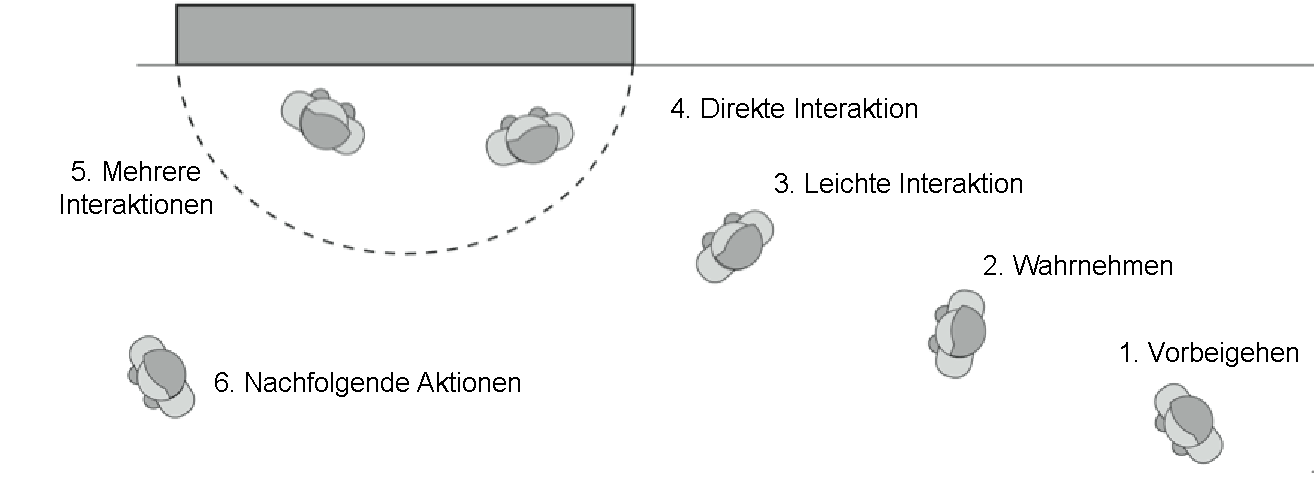
\includegraphics[width=0.8\textwidth]{audiencefunnel.pdf}
    \end{center}
    \caption{Audience Funnel Framework. Abbildung aus \citet{mai_audience_2018}.}
    \label{fig:AudienceFunnelModel}
  \end{figure}

Ein zweites Modell wird durch den bereits erwähnten \emph{Honeypot-Effekt} beschrieben.
Er zeigt, dass Individuen unabhängig von Belohnung, Bestrafung oder sozialem Wettbewerb
von der reinen Präsenz oder den Aktivitäten anderer beeinflusst werden \citep{wouters_uncovering_2016}..
In der \ac{HCI} wird dies meist erkennbar, indem Passanten sich einem System nähern
und überlegen, ob sie mit ihm interagieren sollen,
nachdem sie anderen Menschen dabei zugesehen haben \citep{wouters_uncovering_2016}.

Eine Einordnung der Bewegungsdaten in die Kategorien solcher Modelle
und eine weiterführende Analyse der Bewegungen kann Aufschluss über das Verhalten von Menschen
vor interaktiven Bildschirmen geben.
Wie bereits erwähnt, soll eine derartige Kategorisierung automatisiert werden.

\section{Spezifikation der Kinect}
\label{2-SpezifikationKinect}
Ursprünglich war der Xbox 360 Kinect-Sensor ausschließlich für die Videospiel-Industrie gedacht.
Schon bald wurde dieser aber auch für wissenschaftliche Experimente genutzt \citep{tolgyessy_evaluation_2021}.
So kam auch im vorliegenden Datensatz des \emph{HoPE-Projekts} die Kinect v2 für Xbox One zum Einsatz.
Die zugrunde liegende Sensorik stellt Farbbilder einer \ac{RGB} Kamera, Tiefendaten mithilfe einer Tiefenkamera
und Audiodateien verschiedener Mikrofone zur Verfügung \citep{windows-developer-center_microsoft_corporation_human_2014}.
Tiefenkameras ordnen jedem Punkt eines Bildes eine Entfernung zum Sensor zu.
Dies hilft zuverlässige Ergebnisse bei der Erkennung von Menschen vor \emph{Ambient Displays} zu erzielen.
\citet{li_time-flight_2014} stellen fest:
\glqq Die kompakte Größe, die Benutzungsfreundlichkeit,
die stark vereinfachte Hintergrund-Subtraktion im Vergleich zu anderer Sensorik, sowie die hohe Genauigkeit
und die hohe Bildrate machen Tiefenkameras zu einer attraktiven Lösung für ein breites Spektrum an Anwendungen.\grqq\
Die Kinect v2 verwendet dabei den Ansatz der kontinuierlichen Wellenintensitätsmodulation,
der häufig bei \ac{ToF}-Tiefenkameras zum Einsatz kommt.
Dabei wird das Licht einer Lichtquelle von anderen Objekten im Sichtfeld der Kamera zurückgestreut
und die Zeit zwischen der Emittierung und dem Wiedereintreffen des reflektierten Licht gemessen.
Im weiteren Verlauf wird diese \glqq Flugzeit\grqq\ für jedes Pixel im Bild in einen Entfernungswert umgerechnet \citep{tolgyessy_evaluation_2021}.
Der Sensor kann Tiefenbilder mit einer Auflösung von 512 x 424 Pixeln
und Farbbilder mit 1920 x 1080 Pixeln aufnehmen \citep{marin_multi-camera_2019}.
Bei der Kinect v2 können bis zu sechs Personen erfasst werden.
Dabei wird die Lage von 25 Skelettpunkten, sowie verschiedene Gesichtsattribute erfasst \citep{windows-developer-center_microsoft_corporation_human_2014}.
\autoref{fig:KinectBodyJoints} zeigt eine Übersicht dieser Punkte. 
\begin{figure}[ht]
  \begin{center}
  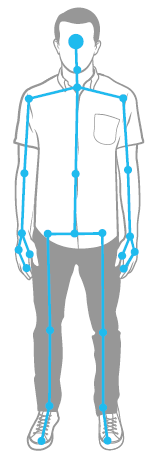
\includegraphics[width=0.1\textwidth]{kinect-body-joints.png}
  \end{center}
  \caption{Skelettpunkte der Kinect v2. Abbildung von \citet{windows-developer-center_microsoft_corporation_human_2014}.}
  \label{fig:KinectBodyJoints}
\end{figure}

\section{Struktur des vorliegenden Datensatzes}
\label{2-StrukturDatensatz}
Im Rahmen eines Feldeinsatzes wurden im Jahr 2017 Ambient Displays für 18 Wochen mit Kinect v2 Systemen ausgestattet \citep{schwarzer_spontaneous_2021}.
Der dabei entstandene Datensatz dient zur späteren Evaluation der zu implementierenden Anwendung.

Eine Betrachtung des Datensatzes ergab, dass dieser 97.626 Records beinhaltet \citep{temiz_konzeption_2022}.
Dabei sind jedem Record mehrere sogenannte Frames zugeordnet,
welche der Momentaufnahme eines Menschen entsprechen.
Jede Person erhält eine eindeutige Identifikationsnummer.
Falls sich mehr als eine Person gleichzeitig im Sensorbereich befindet,
erfolgt eine weitere Unterteilung des Records in Frames \citep{temiz_konzeption_2022}.
Zu jedem Record liegen verschiedene Dateien vor.
Sie tragen jeweils den Zeitstempel in Kombination mit einem geeigneten Postfix als Dateinamen.
\autoref{tbl:AttributesDataset} zeigt die Attribute der Datei \emph{timestamp.txt}.
Diese Attribute können im Kontext der Kategorisierung von Bewegungsdaten genutzt werden.
Dazu kann eine Teilmenge der Werte verschiedener Records miteinander verglichen werden.
So können sie auf Gemeinsamkeiten und Unterschiede hin untersucht werden.
Die Attribute werden in der Textdatei durch das Trennzeichen '\#\#\#' voneinander abgegrenzt.
Ein exemplarischer Frame aus dem Datensatz kann \autoref{fig:FrameExample} entnommen werden.
Da die Anordnung und das Vorhandensein dieser Attribute je nach Version des Datensatzes abweichen kann,
sollen diese in der Implementierung manuell konfigurierbar sein.
Selbes gilt für das Trennzeichen.
Das Tool kann deshalb auch eingesetzt werden,
falls verschiedene Versionen des Datensatzes ausgeliefert wurden.
Die Datei \emph{timestamp$\_$bodies.txt} enthält für jeden Frame die Position aller 25 Skelettpunkte.
\emph{timestamp.xef} kann genutzt werden, um die Aufnahme in der Anwendung Kinect Studio zu visualisieren.
Letztlich sind die Einträge sogenannte \emph{\ac{TSD}}.
Bei diesem Datentyp handelt es sich um geordnete Sequenzen von Datenpunkten,
die, oft in regelmäßigen Abständen, über eine gewisse Zeit hinweg aufgenommen wurden \citep{ali_clustering_2019}.
Insgesamt befinden sich im Datensatz 34.687.630 Frames \citep{temiz_konzeption_2022}.
Diese Anzahl verdeutlicht die Notwendigkeit eines Software-Tools zur Auswertung.
Für diese Bachelorarbeit wurde eine vorselektierte Version des Datensatzes bereitgestellt,
welche auch in \autoref{chapter6} zum Einsatz kommt.
Dieser Datensatz kam durch folgende Regeln zustande:
\begin{enumerate}
  \item Nur Aufzeichnungen von Werktagen werden beachtet.
  \item Nur Aufzeichnungen zwischen 07:00 Uhr und 17:59 Uhr werden beachtet.
  \item Nur Aufzeichnungen mit mindestens 63 Frames pro Aufzeichnung werden beachtet.
  \item Nur Aufzeichnungen mit Personen, die Mindestmaß an Aufmerksamkeit zeigen, werden beachtet.
  \item Aufzeichnungen mit 100 Prozent Engagement werden nicht beachtet, da manche dieser Fälle durch die Kinect falsch erkannt wurden.
  \item Aufzeichnungen mit großen Sprüngen auf den Achsen werden nicht beachtet.
\end{enumerate}
Hier ist anzumerken, dass das zu entwickelnde Tool auch mit anderen Datensätzen funktionieren soll.
So sollen bei Bedarf zum Beispiel auch Daten anderer Tiefenkameras geclustert werden können.
\begin{table}[ht]
  \begin{center}
    \begin{tabular}{ |c|c| } 
      \hline
      Attributname & Beschreibung \\
      \hline \hline
      Zeitstempel & Zeitpunkt der Aufnahme. \\
      \hline
      KinectId & Skelett-Identifikationsnummer des Frameworks.  \\
      \hline
      RecordId & Identifikationsnummer des Records. \\
      \hline
      BodyIndex & Identifikationsnummer der Person. \\
      \hline
      BodyCount & Anzahl der erfassten Personen. \\
      \hline
      Happy & Person ist glücklich. \\
      \hline
      Engaged & Person zeigt Interesse. \\
      \hline
      WearingGlasses & Person trägt eine Brille. \\
      \hline
      LeftEyeClosed & Person hat das linke Auge geschlossen. \\
      \hline
      RightEyeClosed & Person hat das rechte Auge geschlossen. \\
      \hline
      MouthOpen & Person hat den Mund geöffnet. \\
      \hline
      MouthMoved & Person bewegt den Mund. \\
      \hline
      LookingAway & Person schaut nicht zur Kinect. \\
      \hline
      Body.HandLeftState & Zustand der linken Hand. \\
      \hline
      Body.HandRightState & Zusand der rechten Hand. \\
      \hline
      x & x-Koordinate des Skelettpunkts SpineShoulder. \\
      \hline
      y & y-Koordinate des Skelettpunkts SpineShoulder. \\
      \hline
      z & z-Koordinate des Skelettpunkts SpineShoulder. \\
      \hline
      Distance & Distanz zwischen Kinect und SpineShoulder (in Metern). \\
      \hline
    \end{tabular}
    \caption{Attribute des Datensatzes.}
    \label{tbl:AttributesDataset}
  \end{center}
\end{table}
\begin{center}
  \begin{figure}[ht]
    2017-04-10 07:41:53.943 +02:00 \#\#\# 72057594038063128 \#\#\# 1341053376 \#\#\# 1 \#\#\#
    \newline 1 \#\#\# No \#\#\# Maybe \#\#\# Unknown \#\#\# No \#\#\# No \#\#\# No \#\#\# Yes \#\#\#
    \newline Maybe \#\#\# Unknown \#\#\# Closed \#\#\# 0,1074784 \#\#\# 0,2451882 \#\#\# 4,18441 \#\#\#
    \newline 4,19296454679429
    \caption{Frame aus dem Datensatz.}
    \label{fig:FrameExample}
  \end{figure}
\end{center}

\clearpage
\section{Problembeschreibung}
\label{2-Problembeschreibung}
Wesentliches Ziel ist die Kategorisierung von Bewegungsdaten.
Da die Bewegungen von verschiedenen Personen ausgeführt werden,
kann es sein, dass gegebenenfalls auch gleiche Bewegungshandlungen voneinander abweichen.
Zudem kann es vorkommen, dass die Bewegungen zu unterschiedlichen Zeitpunkten in den Records auftreten.
Diese Tatsachen machen eine manuelle Kategorisierung oft schwierig.
Hinzu kommt das bereits beschriebene Problem der großen Datenmenge.
Im Folgenden sollen mögliche Lösungsansätze der beschriebenen Problematik diskutiert werden.

Es gibt verschiedene Möglichkeiten sich der Kategorisierung von Bewegungsdaten zu nähern \citet{aghabozorgi_time-series_2015}.
So kann beispielsweise der Ansatz des \emph{Maschine Learning} eingesetzt werden,
welcher derzeit ebenfalls im Rahmen des HoPE-Projekts erforscht \citep{plischke_master_2022} wird.
In dieser Bachelorarbeit werden hingegen \emph{deterministische Algorithmen} genutzt.
\citet{aghabozorgi_time-series_2015} verweisen darauf, dass die Verwendung von Methoden
wie Maschine Learning (\emph{supervised}), im Falle von großen Datensätzen, zu Problemen führen kann.
Es ist nicht möglich Trainingsdaten, die alle möglichen Szenarien abdecken, zur Verfügung zu stellen.
Dies ist auch nicht Ziel der Untersuchungen.
Stattdessen soll geprüft werden,
ob mithilfe der Anwendung Bewegungsabläufe automatisiert gefunden werden können.
\emph{Deterministische Cluster-Algorithmen} sind hier geeignet,
da diese keine zuvor definierten Klassen benötigen \citep{aghabozorgi_time-series_2015}.

Ziel der Verarbeitung ist es, möglichst sinnvolle \emph{Cluster} zu erhalten.
Um die Gemeinsamkeiten zweier Aufnahmen zu berechnen,
wird eine geeignete Vergleichsfunktion benötigt.
Die Wahl dieser Funktion ist ausschlaggebend für den Erfolg des \emph{Clusterings} \citep{warren_liao_clustering_2005}.
Zu beachten ist zudem, dass die Bewegungsaufnahmen durch \ac{TSD} beschrieben werden.
Bei der bloßen Anwendung herkömmlicher Distanzmetriken, wie der Euklidische-Distanz,
ist die Aussagekraft des Vergleichs gering \citep{warren_liao_clustering_2005}.
Wie bereits erwähnt kann es vorkommen, dass verschiedene Personen die gleiche Bewegung unterschiedlich schnell,
oder zeitlich versetzt ausführen.
Gegebenenfalls weisen die Datenreihen gleicher Bewegungen daher sogar eine unterschiedliche Anzahl an Frames auf.
Dies wird in \autoref{fig:MetricComparison} veranschaulicht.
\begin{figure}[ht]
    \begin{center}
    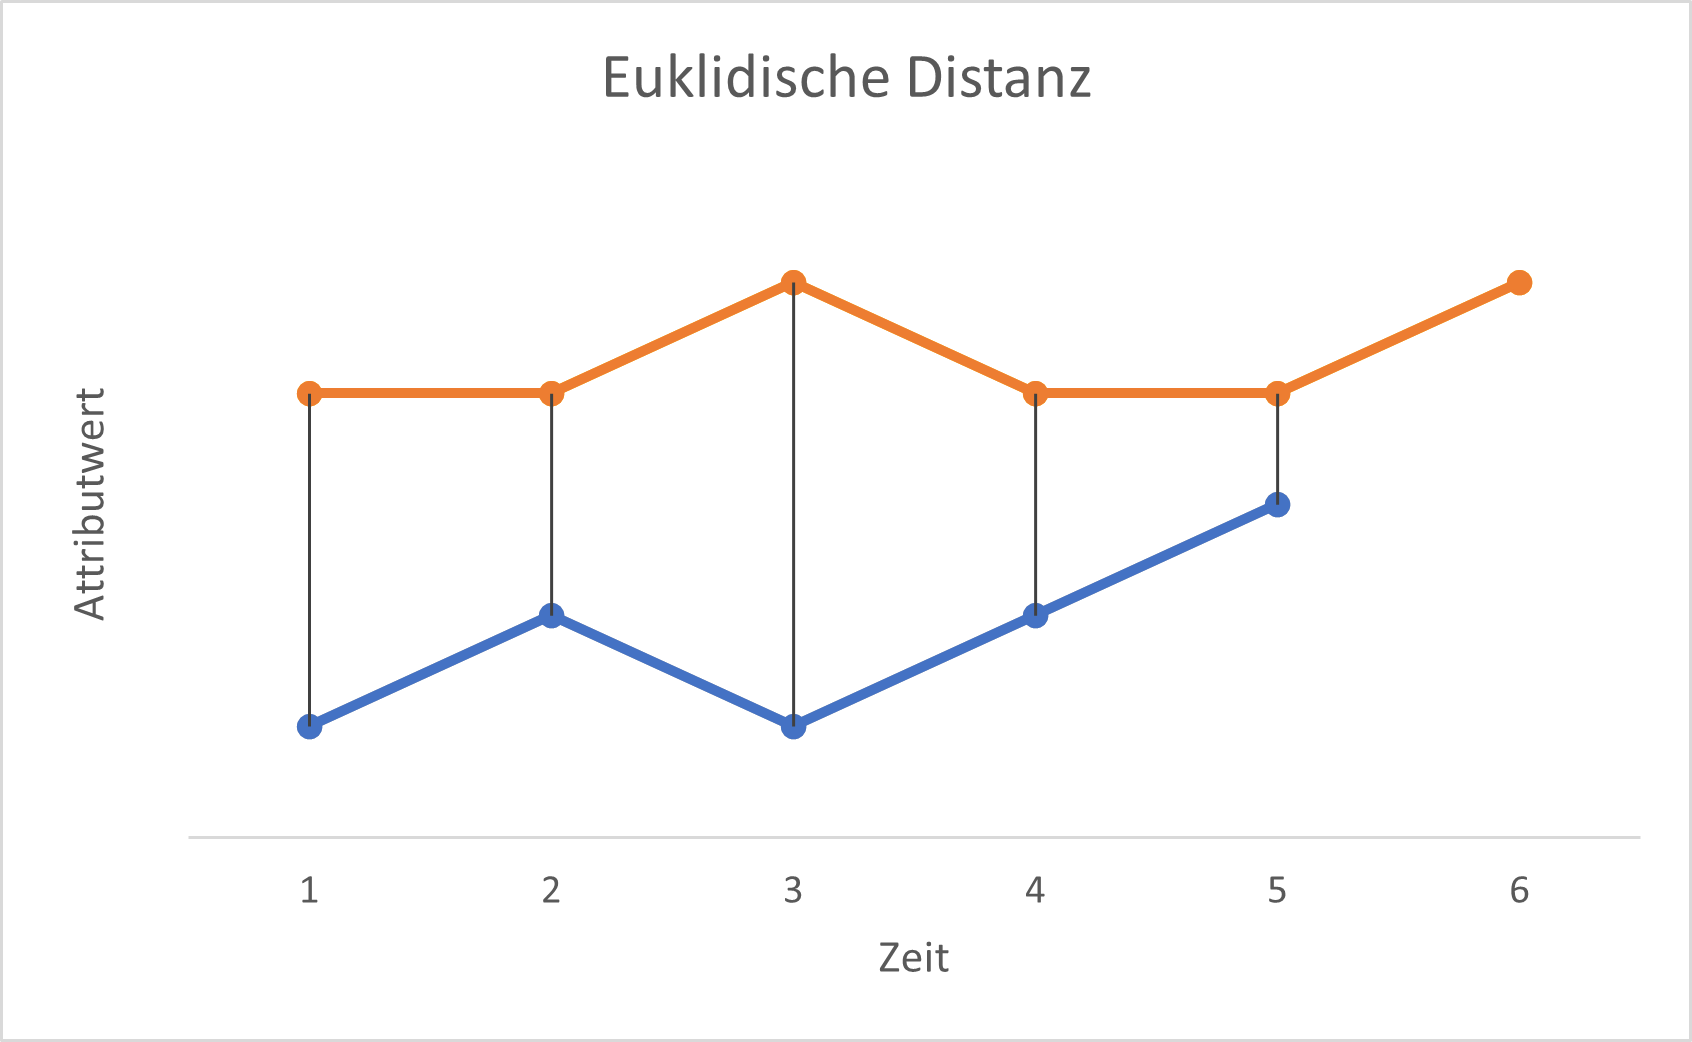
\includegraphics[width=0.45\textwidth]{EuclidianMetric.png}
    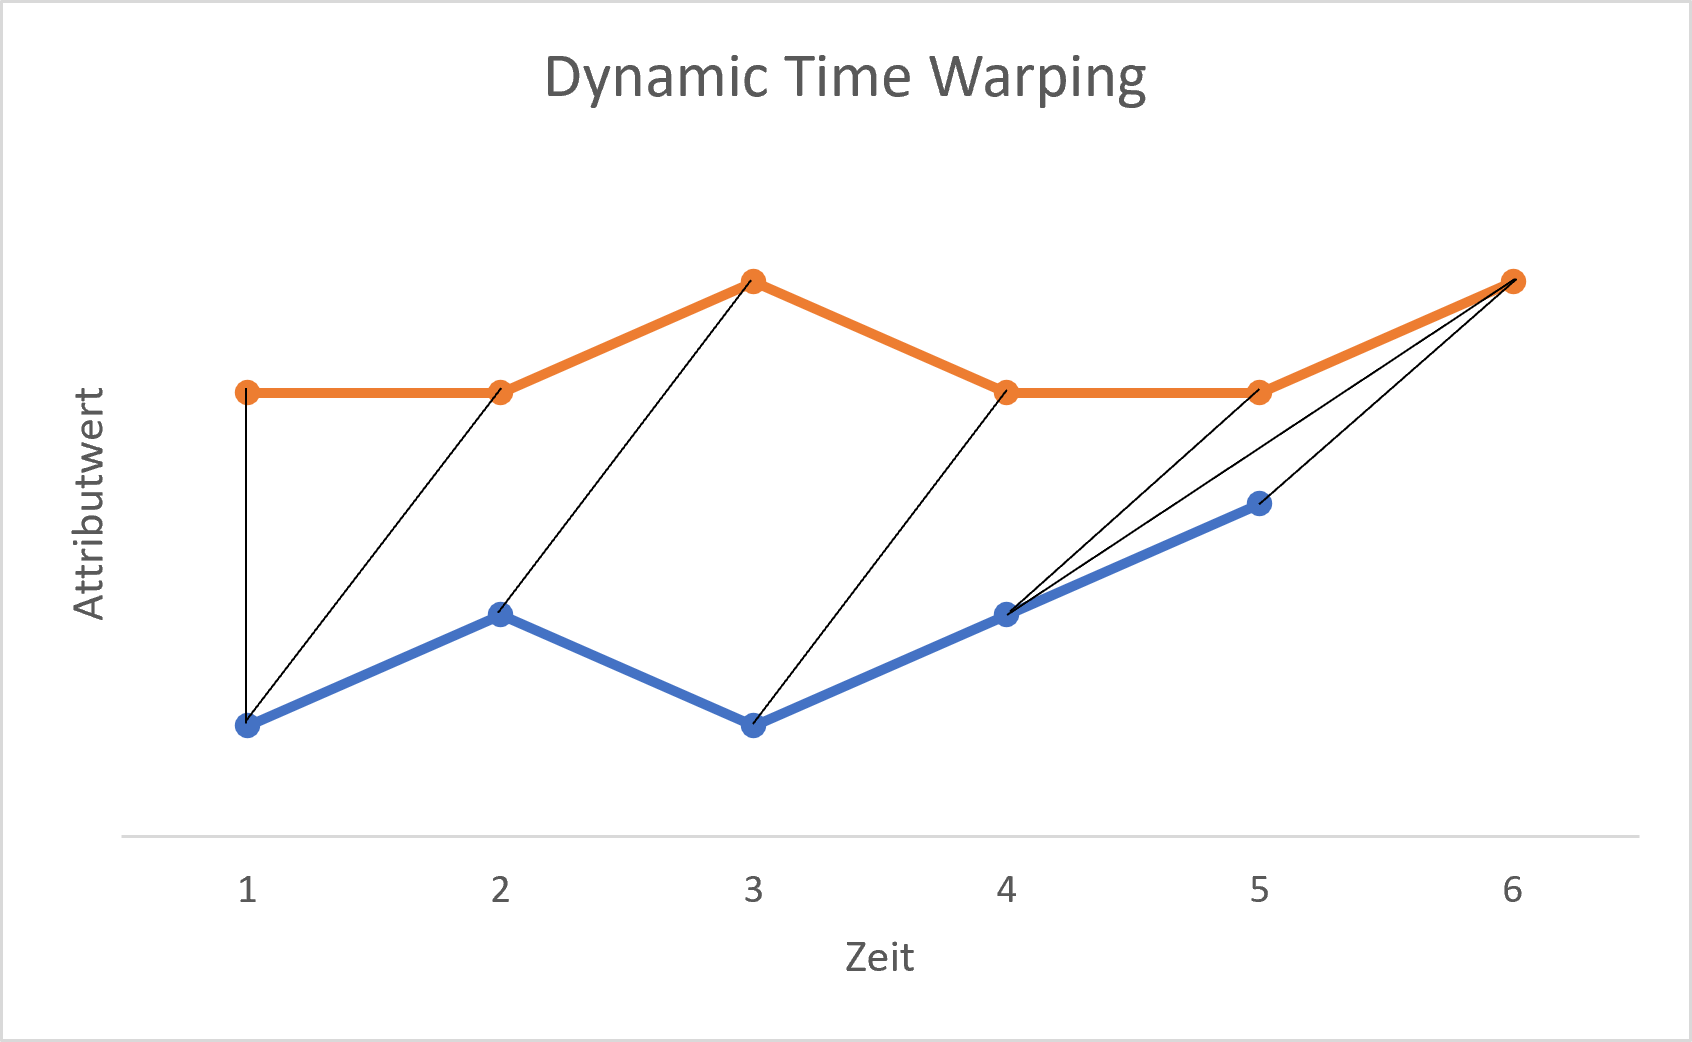
\includegraphics[width=0.45\textwidth]{DTWMetric.png}
    \end{center}
    \caption{Zuordnung der Messpunkte zweier Datenreihen.}
    \label{fig:MetricComparison}
\end{figure}
Die Kurven weisen ähnliche Segmente auf.
Diese Ähnlichkeiten treten allerdings zu unterschiedlichen Zeitpunkten auf.
Zudem sind die Datenreihen unterschiedlich lang.
Der letzte Punkt der Reihe kann daher gar keinem anderen Punkt zugordnet werden.
Bei der bloßen Anwendung der bekannten euklidischen Distanz,
ohne Zuordnung der Punkte, ist das Ergebnis hier gegebenenfalls nicht aussagekräftig.
Um dieses Problem zu lösen ist eine \emph{elastische Metrik} nötig,
die besser mit zeitlichen Verschiebungen umgehen kann \citep{aghabozorgi_time-series_2015}.
Dazu wird \emph{\ac{DTW}} verwendet (\autoref{3-DTW}).
Hier ist eine Mehrfachzuordnung von Punkten möglich.
Dies erlaubt eine Zuordnung ähnlicher Muster in den Daten, auch wenn sie zeitlich verschoben sind \citet{mohammadzade_dynamic_2021}.
Diese können so verbunden werden, dass die Kombinationskosten minimal sind.
Es gibt also keine andere Zuordnung der Punkte,
sodass die Summe der Differenzen zwischen ihnen geringer ist.
Das Clustering soll mithilfe von \emph{hierarchischem Clustering},
welches in \autoref{3-Clustering} beschrieben wird, durchgeführt werden.
Das Verfahren ist für die vorliegenden Daten geeignet,
da es erlaubt \ac{TSD} unterschiedlicher Länge zu clustern.
Zudem muss die Anzahl der zu bildenden Cluster nicht im Voraus definiert werden,
wie dies etwa bei \emph{K-Means} der Fall ist \citep{aghabozorgi_time-series_2015}.
Es ist in diesem Kontext nicht zielführend die Clusteranzahl zuvor zu definieren,
da die Arbeit darauf abzielt, mehr Erkenntnis über mögliche sinnvolle Cluster zu gewinnen.
Statt die Anzahl vorzugeben, wird ein \emph{Threshold} definiert der angibt,
ab wann zwei Cluster nicht mehr zusammengeführt werden sollen,
weil die Differenz zwischen ihnen zu groß ist.
Hierarchisches Clustering mit \ac{DTW} ist also zur Lösung des beschriebenen Problems geeignet.